\documentclass[aspectratio=169,11pt]{beamer}
\usepackage{teaching_slides}
\usepackage{listings}

\lstset{
  language=R,
  basicstyle=\ttfamily\tiny,
  backgroundcolor=\color{gray!5},
  frame=single,
  rulecolor=\color{gray!50},
  keywordstyle=\color{blue!70!black},
  commentstyle=\color{green!40!black},
  stringstyle=\color{orange!90!black},
  columns=flexible,
  keepspaces=true,
  showstringspaces=false,
  breaklines=true
}


\usepackage{inconsolata} % nice monospace font


\title{Program Evaluation and Randomized Experiments}
\author{Chris Conlon}
\institute{Applied Econometrics}
\date{\today}

\begin{document}


\frame{\titlepage}

\frame{\frametitle{Overview}
This set of lectures will cover (roughly) the following papers:\\
Theory:
\begin{itemize}
\item Angrist and Imbens (1994)
\item Heckman Vytlacil (2005/2007)
\item Abadie and Imbens (2006)
\end{itemize}
And draw heavily upon notes by 
\begin{itemize}
\item Guido Imbens
\item Richard Blundell and Costas Meghir
\end{itemize}

}

\begin{frame}
\frametitle{The Evaluation Problem}
\begin{itemize}
\item The issue we are concerned about is identifying the effect of a policy or an investment or some individual action on one or more outcomes of interest
\item This has become the workhorse approach of the applied microeconomics fields (Public, Labor, etc.)
\item Examples may include:
\begin{itemize}
\item The effect of taxes on labor supply
\item The effect of education on wages
\item The effect of incarceration on recidivism
\item The effect of competition between schools on schooling quality
\item The effect of price cap regulation on consumer welfare
\item The effect of indirect taxes on demand
\item The effects of environmental regulation on incomes
\item The effects of labor market regulation and minimum wages on wages and employment
\end{itemize}
\end{itemize}
\end{frame}

\begin{frame}{Potential Outcomes}
\begin{itemize}
\item Consider a binary treatment $D_i \in \{0,1\}$. 
\begin{itemize}
\item Some people use $T_i \in \{0,1\}$ instead.
\end{itemize}
\item We observe the outcome $Y_i$. But there are two \alert{potential outcomes}
\begin{itemize}
\item $Y_i(1)$ the outcome for $i$ if they  \alert{are treated}.
\item $Y_i(0)$ the outcome for $i$ if they \alert{are not treated} (control).
\end{itemize}
\item We are generally interested in $\beta_i \equiv  Y_i(1)-Y_i(0)$ which we call the \alert{treatment effect}.
\begin{itemize}
\item Individuals have \alert{heterogeneous treatment effects}.
\item In an ideal world we could fully characterize $f(\beta_i)$
\end{itemize}
\end{itemize}
\end{frame}

\begin{frame}{Some Challenges}
Stable unit treatment value assumption (SUTVA)
\begin{itemize}
\item We assume a \textit{ceteris paribus} version of treatment effects
\item We need $\beta_i$ to be a policy invariant (structural) parameter.
\item Your $\beta_i$ doesn't respond to whether or not another individual is treated.
\item Two common limitations:
\begin{itemize}
\item Peer effects: Whether you respond to job training program depends on whether your spouse is also treated.
\item Equilibrium effects: if we sent everyone to college, returns to college would be quite different.
\end{itemize}
\end{itemize}
\end{frame}



\begin{frame}{Some Challenges}
\begin{columns}[T] % align columns
\begin{column}{.65\textwidth}
Fundamental Problem of Causal Inference
\begin{itemize}
\item We don't observe the \alert{counterfactual} $Y_i(D_i)$.
\item For a single individual we either observe $Y_i(1)$ \alert{or} $Y_i(0)$ but never both!
\begin{itemize}
\item ex: We don't see what your wage would have been if you didn't attend college.
\item ex: We might know your cholesterol before you took Lipitor, but we don't know what it would be today if you didn't take Lipitor.
\end{itemize}
\end{itemize}
\end{column}%
\hfill%
\begin{column}{.38\textwidth}

  \vspace{20pt}
  
  $Y_{i} = D_{i}\cdot Y_{i}(1) + (1-D_{i}) \cdot Y_{i}(0)$\\
  \vspace{20pt}
  \begin{tabular}{ccccc}
    \toprule
    i & $Y_{i}(1)$ &  $Y_{i}(0)$ & $D_{i}$ & $D_{i}$ \\
    \midrule
    1 &     1      &     \alert{?}      &   1   & 1 \\
    2 &     0      &     \alert{?}      &   1   & 0 \\
    3 &     \alert{?}      &     0      &   0   & 0 \\
     & &  $\vdots$ & & \\
    $n$ &     \alert{?}      &     1      &   0   & 1 \\    
  \end{tabular}
\end{column}%
\end{columns}
\end{frame}


\begin{frame}
\frametitle{Structural vs. Reduced Form}
\begin{itemize}
\item Usually we are interested in one or two parameters of the distribution of $\beta_i$ (such as the average treatment effect or average treatment on the treated).
\item Most program evaluation approaches seek to identify one effect or the other effect. This leads to these as being described as \alert{reduced form} or \alert{quasi-experimental}.
\item The \alert{structural} approach attempts to recover the entire joint $f(\beta_i,\varepsilon_i)$ distribution but generally requires more assumptions, but then we can calculate whatever we need.
\end{itemize}
\end{frame}


\begin{frame}
\frametitle{Treatment Effects Parameters}
Most approaches to estimating treatment effects will recover some moments of $f(\beta_i)$ instead of the entire distribution
\begin{description}
\item[Average Treatment Effect (ATE)] corresponds to $\E[\beta_i]$.
\item[Average Treatment on Treated (ATT)] corresponds to $\E[\beta_i \mid D_i = 1]$.
\item[Average Treatment on Control/Untreated (ATUT)] corresponds to $\E[\beta_i \mid D_i = 0]$.
\end{description}
We also have that if the probability of treatment $\Pr(D_i=1) = \pi$
\begin{align*}
ATE = \pi \cdot ATT + (1-\pi) \cdot ATUT
\end{align*}
\end{frame}


\begin{frame}
\frametitle{The Selection Problem}
\begin{itemize}
\item Let's start with the easy cases: run OLS and see what happens.
\begin{align*}
Y_i = \alpha + \beta_i \cdot D_i + \varepsilon_i
\end{align*}
\item OLS compares mean of treatment group with mean of control group (possibly controlling for other $X$)
\begin{eqnarray*}
\beta^{OLS} &=& \E(Y_i \mid D_i =1) - \E(Y_i \mid D_i=0) \\
&=& \underbrace{\E[\beta_i \mid  D_i =1]}_{\mbox{ATT}} + \left(\underbrace{\E[\varepsilon_i \mid D_i =1 ] - \E[\varepsilon_i \mid D_i=0] }_{\mbox{selection bias}}  \right)
\end{eqnarray*}
\item Even in absence of heterogeneity $\beta_i = \beta$ we can still have selection bias. 
\item $Y_i^0 = \alpha + \varepsilon_i$ may vary within the population (this is quite common).
\end{itemize}
\end{frame}

\begin{frame}
\frametitle{Why worry about selection?}
Unless we have random assignment...
\begin{align*}
Y_i = \alpha + \beta_i D_i + u_i
\end{align*}

\begin{itemize}
\item People often choose $D_i$ with $\beta_i$ in mind.
\item The problem: $D_i \perp u_i$ and/or $D_i \perp \beta_i$ are likely violated.
\item We can get positive or negative selection bias:
\begin{itemize}
\item e.g. Who goes to college? those likely to benefit more than most!
\item e.g. who gets risky surgeries/drugs? people who are very sick.
\end{itemize}
\end{itemize}
\end{frame}


\begin{frame}{The Magic of Randomization}
\begin{align*}
\begin{array}{ccc}
\E\left[Y_{i}(1) \mid D_{i}=1\right]-\E\left[Y_{i}(0) \mid D_{i}=0\right] & =\\
\E\left[Y_{i}(1) \mid D_{i}=1\right]-\E\left[Y_{i}(0) \mid D_{i}=1\right] & + & \underbrace{\E\left[Y_{i}(0) \mid D_{i}=1\right]-\E\left[Y_{i}(0) \mid D_{i}=0\right]}\\
 &  & \text{selection bias}
\end{array}
\end{align*}
\begin{itemize}
  \item If treatment is assigned randomly, then $Y_{i}(0)$ and $T_{i}$ should be independent. Consequently,
  \begin{align*}
    \E\left[Y_{i}(0)\mid D_{i}=1\right]=\E\left[Y_{i}(0) \mid D_{i}=0\right],
  \end{align*}
recalling that if $Y_{i}(0)$ and $D_{i}$ are independent, $\E\left[Y_{i}(0) \mid D_{i}\right]=\E\left[Y_{i}(0)\right]$.

\item Thus, randomization of treatment eliminates selection bias.
\end{itemize}
\end{frame}


\begin{frame}{The Magic of Randomization II}
\begin{itemize}
  \item We've just shown that randomization gives us the average effect of treatment on the treated (ATT)
  without selection bias.
  \begin{align*}
    \E\left[Y_{i}(1) \mid D_{i}=1\right]-\E\left[Y_{i}(0) \mid D_{i}=0\right]=\E\left[Y_{i}(1)\mid D_{i}=1\right]-\E\left[Y_{i}(0) \mid D_{i}=1\right]
  \end{align*}

  \medskip
  \item Furthermore, randomization of treatment also implies that the ATT equals
  the ATE. If $D_{i}$ is independent of $Y_{i}(0)$ and $Y_{i}(1)$, then
  \begin{align*}
\E\left[Y_{i}(1) \mid D_{i}=1\right]-\E\left[Y_{i}(0) \mid D_{i}=1\right]
&=\E\left[Y_{i}(1)\right]-\E\left[Y_{i}(0)\right]\\
&= \E\left[Y_{i}(1) - Y_{i}(0)\right].
\end{align*}

\end{itemize}
\end{frame}

\begin{frame}{What Does Randomization Do?}
\begin{enumerate}
  \item Randomization of treatment eliminates selection bias.

  \item Randomization of treatment ensures that the ATE=ATT.
\end{enumerate}
\end{frame}


\begin{frame}{Randomization and Endogeneity I}
\begin{itemize}
  \item Selection bias has to do with the fact that \emph{baseline} outcomes for the treated
  and untreated groups may differ. Example: schoolchildren who get the treatment of having
  small class sizes (private schools) are also children who have access to private tutors and well-educated parents.

  \medskip
\item This is a version of an \emph{endogeneity} problem, and it's a fundamental problem for causal inference.
  Randomizing treatment solves the problem, for it means that baseline outcomes should no longer be correlated with the treatment.
\end{itemize}
\end{frame}

\begin{frame}{Randomization and Endogeneity II}
\begin{itemize}
  \item Simplifying the situation by assuming $\beta=Y_{i}(1)-Y_{i}(1)$ for all
$i$, we can put this back in the regression equation framework,
\begin{align*}
Y_{i}=\beta_{0}+\beta_{1}\, D_{i}+\varepsilon_{i}
\end{align*}
where $\beta_{0}=\E\left[Y_{i}(0)\right]$ and $\varepsilon_{i}=Y_{i}(0)-\beta_{0}$.

  \medskip
  \item If heterogeneity in baseline outcomes  $Y_{i}(0)$  is correlated with treatment status $D_i$,
  then the error term $\varepsilon_{i}$ is correlated with the regressor $\varepsilon_i$,
  violating the strict exogeneity assumption, and leading to biased estimates of $\beta$.

  \medskip
  \item In theory, randomization of regressors is a way of ensuring that the strict exogeneity assumption holds:
  we randomly control $D_i$ so that it won't be related to whatever is in $\varepsilon_i$.
\end{itemize}
\end{frame}

\begin{frame}{Randomization and Endogeneity III}
\begin{itemize}
  \item In practice, randomization doesn't \emph{guarantee} there is no endogeneity problem:
  \begin{itemize}
    \item Random control of treatment may be imperfect: attrition and manipulation.
    \item Treatment status may directly influence $\varepsilon$ in some cases: placebo effects 
      and behavioral responses to treatment. 
    \item Blind and double-blind studies aim to mitigate these concerns.
  \end{itemize}
    
\medskip
  \item This requires more notation to discuss within the potential outcome framework -- we need to distinguish
  between whether subject \emph{believes} they are being treated or not, as well as whether they are \emph{actually}
  being treated or not -- but it is easier to talk about in the regression framework. 
\end{itemize}
\end{frame}


\begin{frame}{Randomization and Endogeneity IV}
\begin{itemize}
  \item What does it mean for the disturbance to be influenced by a regressor? 
  Can't we just consider this an effect of the regressor?
  
  \medskip
  \item It depends: often there will be an external validity issue, in the sense that
  the effect won't extrapolate outside of the study.
  
  \medskip
  \item Examples:
  \begin{itemize}
    \item With placebo effect, we could understand this as treatment influencing the
    disturbance term, but maybe we're happy to enjoy the placebo effect. On the other hand,
    what if we're considering whether to add a nutrient to a pill or not, rather than deciding
    whether or not to give the subjects a pill or not? Perhaps we won't get the placebo effect twice. 
    
    \item If treatment influences error term because of manipulation on the part of the researcher
    implementing the study, then the relationship between treatment and outcomes we see
    typically won't extrapolate outside of the study. {\bf Very important to avoid this!}
  \end{itemize}
\end{itemize}
\end{frame}





\begin{frame}{Randomization and Heterogeneity}
\begin{itemize}
  \item The fact that ATE$\ne$ ATT is a separate issue having to do with \emph{heterogeneity} of treatment effects.
  This issue is also ``solved'' by randomization in a way, but is this an issue we want to solve?

  \medskip
  \item Example: the people who take anti-depressants benefit more than the people who don't.
  The ATE for a given drug in the whole population might be low, but that doesn't mean the drug is
  ineffective. If the ATE within the group of people diagnosed with depression is high, and the people
  who end up taking the drug fall within that group, the ATT in practice might correspond closely to the sub-population ATE.

  \medskip
  \item Bottom line: differences between ATE and ATT don't reflect problems of causal inference, but they
  reflect the importance of {\bf context} and understanding the population of interest.
   There's a reason clinical trials for new cancer drugs typically focus on people that have cancer.


\end{itemize}
\end{frame}



\begin{frame}{Experiment with Regression Controls}
\begin{itemize}
  \item Consider the model \[
  Y_{i}=\beta_{0}+\beta_{1}\, D_{i}+\boldsymbol{\beta}_2' {\bf X}_i + \varepsilon_{i}
  \]
  where $D_i$ is assigned randomly.

  \medskip
  \item Does controlling for ${\bf X}$ matter in the experimental context? Note that
  even if ${\bf X}$  is omitted from the regression model, there is {\bf no problem of
  omitted variables bias} because $D$ and ${\bf X}$ are uncorrelated.

  \medskip
  \item However, controlling for covariates may improve precision of the estimates,
  especially in small sample sizes where ${\bf X}$ may not be balanced across the treatment
  and control groups.

\end{itemize}
\end{frame}

\begin{frame}{Randomization with Small Samples}
\begin{itemize}
  \item In a finite sample, there's always
  a chance that we end up with subjects that look very different
  across the treatment and control groups.
  \begin{itemize}
    \item For observable characteristics, it is customary to check that
    the two groups have similar means and medians. This is often
    Table 1 in experimental papers.
  \end{itemize}

  \smallskip
  \item What would you do if you randomly assigned subjects to the two groups,
  and, before running the experiment, you notice that characteristics are not
  balanced? Would it be bad to re-randomize?

  \smallskip
  \item Related ideas:
  \begin{itemize}
    \item Student (1938), the t-test guy, argued against randomization in agricultural trials.
    Simple random sampling vs. systematic sampling.
    \item Stratified sampling, clustered sampling, sampling theory.
    \item Chassang et al (2012) explore the idea of {\bf selective trials}.
  \end{itemize}

\end{itemize}
\end{frame}


\begin{frame}{Experiments in the Social Science}
\begin{itemize}
  \item Randomized Controlled Trials have long been the gold standard for research
  in the natural sciences.

  \smallskip
  \item In social sciences, many important questions don't lend themselves well
  to randomization.
  \begin{itemize}
    \item Macroeconomic policy, other large-scale policy issues, especially
    when there are spillovers across markets/countries. E.g., what is global
    impact of EU's decision to implement carbon pricing?
    \item Mergers and antitrust, other situations where regulatory questions highly
     context-specific.
  \end{itemize}

  \smallskip
  \item However, experiments are becoming increasingly popular in some fields
  \begin{itemize}
    \item Lab experiments: behavioral economics
    \item Field experiments: development, labor, education
  \end{itemize}

\end{itemize}
\end{frame}



\begin{frame}{Example: Banerjee et al (2007)}
\begin{itemize}
  \item Background: getting kids into schools in India seemingly had
  unimpressive impacts on educational attainment. School quality
  (educational inputs) is also important.

  \smallskip
  \item Experimental treatment: remedial education. Third and fourth
  grade students identified as at risk for falling behind are assigned
  an extra teacher for two hours/day.
  \begin{itemize}
    \item Group A (50\% of schools): third grade classrooms treated
    in 2001-2, fourth grade classrooms treated in 2002-3
    \item Group B (50\% of schools): fourth grade classrooms
    treated in 2001-2, third grade classrooms treated in 2002-3.

\end{itemize}
  \item Note that this experiment design allows for the estimation of several
  treatment effects. 

\end{itemize}
\end{frame}


\begin{frame}{Example: Banerjee et al (2007)}
\begin{center}
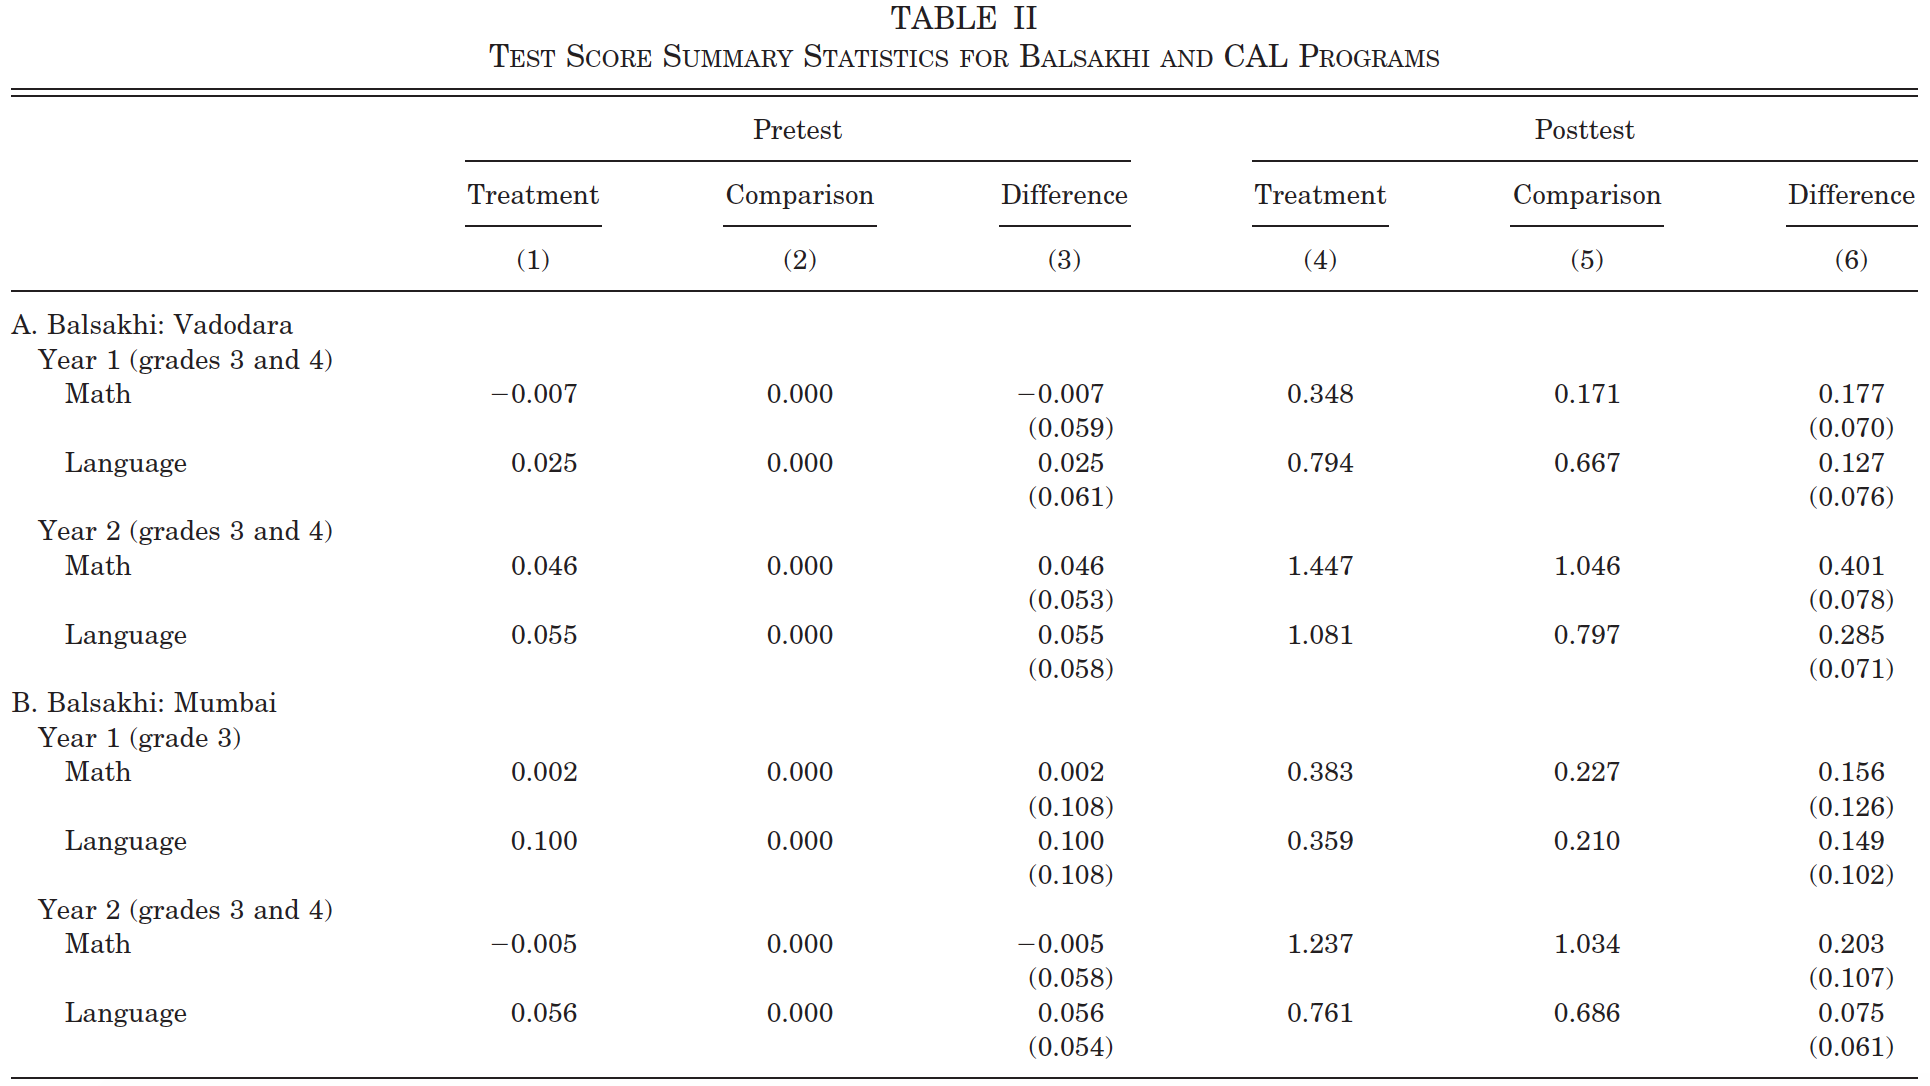
\includegraphics[width=.9\textwidth]{banerjee-t2}
\end{center}
\end{frame}


\begin{frame}{But don't get too excited}
\begin{center}
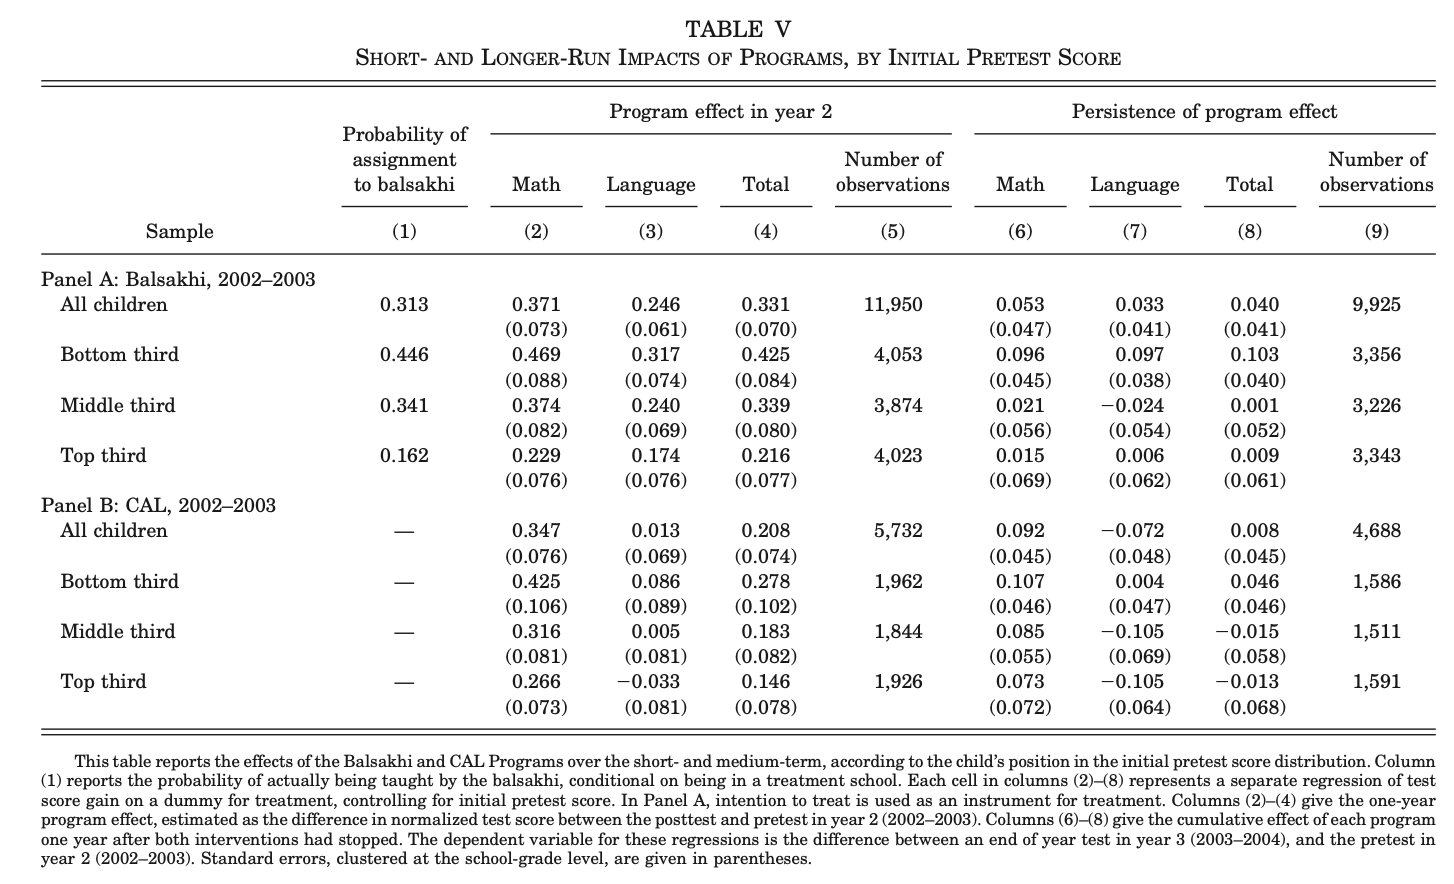
\includegraphics[width=.9\textwidth]{banerjee-t5}
\end{center}
\end{frame}


\section{Designing Randomized Experiments}


\begin{frame}{Nightmare Scenario}
\begin{itemize}
\item You spend big money running an RCT in the field.
\begin{itemize}
  \item You \alert{recruit} your sample
  \item You \alert{pre-register} your statistical analysis
  \item You run your \alert{experiment} and collect your data
  \item Congratulations, you increased the probability of your outcome by 15\% from 1\% to 1.15\%
  \item However, is your sample large enough for a \alert{statistically significant} effect? (Often no!)
\end{itemize}
\end{itemize}
\end{frame}



\begin{frame}{Goal}
  \begin{itemize}
    \item Design an A/B test (randomized experiment) to measure \textbf{lift} from an online ad campaign.
    \item Typical outcome: user-level \textbf{conversion} (binary) or continuous metric (revenue per user, spend).
    \item Decide sample size per arm $n$ for target Type I error $\alpha$ and power $1-\beta$.
  \end{itemize}
\end{frame}

\begin{frame}{Define the estimand: lift}
  \begin{itemize}
    \item Baseline conversion rate (control): $p_0$.
    \item Treatment conversion rate: $p_1$.
    \item Absolute lift: $\Delta = p_1 - p_0$.
    \item Relative lift (percent): $\text{Lift} = \dfrac{p_1 - p_0}{p_0}$, so $p_1 = p_0(1+\text{Lift})$.
  \end{itemize}
\end{frame}

\begin{frame}{Difference in Binary Outcomes (Wald Test)}

Let $\hat{p}_1$ and $\hat{p}_0$ be the sample proportions of succesfful sales in treatment and control.

Under random assignment and large $n_1, n_0$:
\begin{align*}
\hat{p}_j &\sim \mathcal{N}\!\left(p_j,\; \frac{p_j(1-p_j)}{n_j}\right), \quad j\in\{0,1\}
\end{align*}
For large $n$, the difference-in-means is approximately normal:
\begin{align*}
\hat{p}_1 - \hat{p}_0 
\sim \mathcal{N}\!\left(p_1 - p_0,\;
\frac{p_1(1-p_1)}{n_1} + \frac{p_0(1-p_0)}{n_0}\right).
\end{align*}

The Wald test statistic divides by the estimated standard error under $H_0: p_1 = p_0$:
\begin{align*}
Z = \frac{\hat{p}_1 - \hat{p}_0}
         {\sqrt{\hat{p}_1(1-\hat{p}_1)/n_1 + \hat{p}_0(1-\hat{p}_0)/n_0}}
\;\;\xrightarrow[]{d}\;\; \mathcal{N}(0,1)
\end{align*}
This large-sample approximation underpins both the \alert{power} and \alert{sample size} formulas.
\end{frame}


\begin{frame}{Large-sample approx.: two-sample difference-in-proportions}
  Test statistic (Wald) for two independent samples (equal $n$ per arm):
  \begin{align*}
    \hat{p}_1 - \hat{p}_0 \sim \mathcal{N}\!\left(p_1-p_0,\; \frac{p_1(1-p_1)}{n} + \frac{p_0(1-p_0)}{n}\right).
  \end{align*}
  Solving for $n$ to achieve power $1-\beta$ at two-sided significance $\alpha$ gives:
  \begin{align*}
  \begin{aligned}
    n &= \frac{(z_{1-\alpha/2} + z_{1-\beta})^2\;\big(p_1(1-p_1)+p_0(1-p_0)\big)}
               {(p_1-p_0)^2}.
  \end{aligned}
  \end{align*}
  Here $z_{q}$ is the $q$-quantile of the standard normal (e.g. $z_{0.975}\approx 1.96$, $z_{0.8}\approx 0.842$).
\end{frame}

\begin{frame}{Continuous outcome (two-sample t approximation)}
  If the outcome is continuous with (assumed) common variance $\sigma^2$:
  \begin{align*}
    \hat{\mu}_1 - \hat{\mu}_0 \sim \mathcal{N}\!\left(\mu_1-\mu_0,\; 2\frac{\sigma^2}{n}\right)
  \end{align*}
  so
  \begin{align*}
    n = \frac{2\sigma^2\,(z_{1-\alpha/2}+z_{1-\beta})^2}{(\mu_1-\mu_0)^2}.
  \end{align*}
  If you think in terms of standardized effect size $d = \dfrac{\mu_1-\mu_0}{\sigma}$:
  \begin{align*}
    n = \frac{2\,(z_{1-\alpha/2}+z_{1-\beta})^2}{d^2}.
  \end{align*}
\end{frame}

\begin{frame}{Worked example (binary conversion)}
  Suppose:
  \begin{itemize}
    \item Baseline conversion $p_0 = 0.02$ (2\%).
    \item Desired \textbf{relative lift} = 10\% $\Rightarrow p_1 = 0.02 \times 1.10 = 0.022$.
    \item Two-sided $\alpha = 0.05$ and power $1-\beta = 0.80$.
  \end{itemize}

  Compute per-arm sample size from the formula:
  \begin{align*}
  n = \frac{(1.96 + 0.8416)^2\;\big(0.022(1-0.022)+0.02(1-0.02)\big)}{(0.022-0.02)^2}
  \end{align*}
  Numerically this gives
  \begin{align*}
    n \approx 80{,}681 \quad\text{(per arm)}.
  \end{align*}
  \vspace{4pt}
  \textbf{Interpretation:} To detect a 10\% relative increase from a very small base rate (2\%) requires a huge sample because the absolute change is very small (0.2 percentage points).
\end{frame}


\begin{frame}{Alternate example: bigger lift}
  If relative lift = 50\% (so $p_1 = 0.02 \times 1.5 = 0.03$), same $\alpha$ and power:
  \begin{align*}
    n \approx 3{,}823 \quad\text{(per arm)}.
  \end{align*}

\begin{itemize}
  \item So power is very sensitive to the \emph{absolute} difference $p_1-p_0$.
  \item Of course if you knew $p_1$ you wouldn't need to do all this work in the first place!
\end{itemize}
\end{frame}

\begin{frame}[fragile]{R code: compute sample size (binary)}
\begin{lstlisting}
# two-sided test (approx normal)
p0 <- 0.02
lift <- 0.10
p1 <- p0*(1+lift)
alpha <- 0.05
power <- 0.80
z_alpha <- qnorm(1-alpha/2)
z_beta  <- qnorm(power)

n_per_arm <- ((z_alpha + z_beta)^2 * (p1*(1-p1) + p0*(1-p0))) / ((p1 - p0)^2)

ceiling(n_per_arm)
# Alternatively: use power.prop.test for approximation (one-sided/two-sided differences)
power.prop.test(p1 = p0, p2 = p1, power = power, sig.level = alpha,
                alternative = "two.sided")
\end{lstlisting}
\end{frame}




\begin{frame}[fragile]{Calculating the Sample Size/Lift Curve}
\begin{columns}
\begin{column}{0.5\textwidth}
\begin{center}
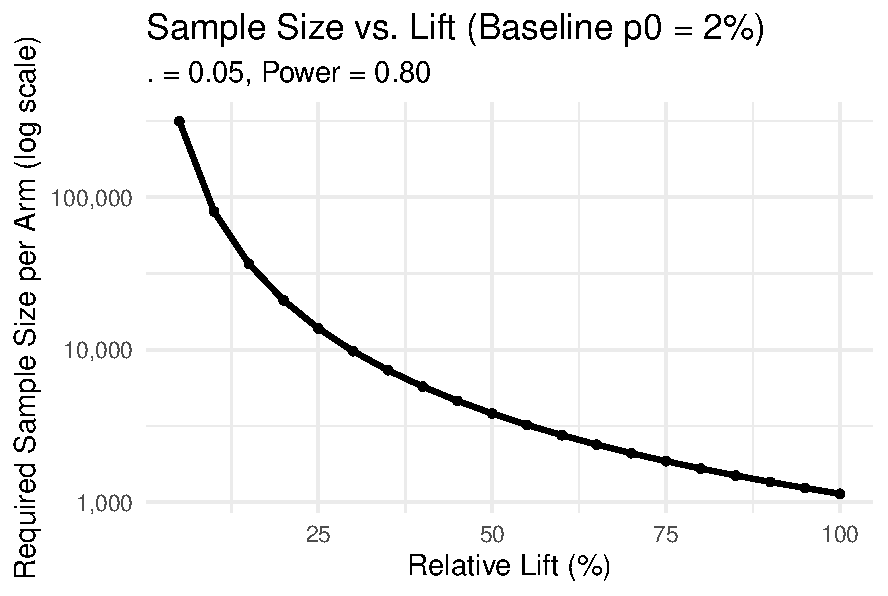
\includegraphics[width=\textwidth]{power_plot} 
\end{center}
\end{column}
\begin{column}{0.5\textwidth} 
\begin{lstlisting}
p0 <- 0.02
alpha <- 0.05
power <- 0.8
z_alpha <- qnorm(1-alpha/2)
z_beta <- qnorm(power)

lift_grid <- seq(0.05, 1.0, by=0.05)
df <- data.frame(
  lift = lift_grid,
  p1 = p0 * (1 + lift_grid)
)
df$n <- ((z_alpha + z_beta)^2 * (df$p1*(1-df$p1) + p0*(1-p0))) / (df$p1 - p0)^2

ggplot(df, aes(x = lift*100, y = n)) +
  geom_line(linewidth=1.2) +
  geom_point() +
  scale_y_log10(labels = scales::comma) +
  labs(
    x = "Relative Lift (%)",
    y = "Required Sample Size per Arm (log scale)",
    title = "Sample Size vs. Lift (Baseline p0 = 2%)",
    subtitle = "α = 0.05, Power = 0.80"
  ) +
  theme_minimal(base_size = 14)
\end{lstlisting}
\end{column}
\end{columns}
\end{frame}




\begin{frame}[fragile]{R code: continuous outcome}
\begin{lstlisting}
# Two-sample t approximation
sigma <- 10.0        # estimated SD of outcome
delta <- 1.0         # desired absolute lift (mu1 - mu0)
alpha <- 0.05
power <- 0.80
z_alpha <- qnorm(1-alpha/2)
z_beta  <- qnorm(power)

n_per_arm <- (2 * sigma^2 * (z_alpha + z_beta)^2) / (delta^2)
ceiling(n_per_arm)

# or use built-in
power.t.test(delta = delta, sd = sigma, power = power,
             sig.level = alpha, type = "two.sample", alternative = "two.sided")
\end{lstlisting}
\end{frame}


\begin{frame}{Minimum Detectable Effect (MDE)}
  Often we have fixed $n$ and want the smallest detectable absolute difference $\Delta$ at given $\alpha, \beta$:
  \begin{align*}
    \Delta = (z_{1-\alpha/2} + z_{1-\beta}) \sqrt{\frac{p_1(1-p_1)+p_0(1-p_0)}{n}}.
  \end{align*}
  For planning you can use the conservative plug-in $p_1\approx p_0$, giving
  \begin{align*}
    \Delta_{\text{approx}} \approx (z_{1-\alpha/2} + z_{1-\beta}) \sqrt{\frac{2 p_0(1-p_0)}{n}}.
  \end{align*}
  Convert to relative lift as $\text{Lift} = \Delta / p_0$.
\end{frame}

\begin{frame}{Practical considerations}
  \begin{itemize}
    \item \textbf{Equal vs unequal allocation:} If treatment fraction $\pi \ne 0.5$, replace $1/n+1/n$ by $1/(n\pi)+1/(n(1-\pi))$ or solve for each arm separately.
    \item \textbf{Clustering / interference:} If randomization is by cluster (e.g., by geography), inflate $n$ by the design effect: $DE = 1 + (m-1)\rho$, where $m$ is cluster size, $\rho$ ICC.
    \item \textbf{Multiple testing / sequential peeking:} Correct $\alpha$ (Bonferroni, group sequential, alpha-spending).
    \item \textbf{Non-compliance / attrition:} Adjust expected treated proportion and effective sample size.
    \item \textbf{Heterogeneous treatment effects:} If variance differs by arm, use $p_1(1-p_1)$ and $p_0(1-p_0)$ explicitly.
    \item \textbf{Pre-launch A/B to estimate $p_0$ and $\sigma$:} Accurate estimates of baseline rate and SD drastically change required $n$.
  \end{itemize}
\end{frame}

\begin{frame}{Quick checklist before running}
  \begin{enumerate}
    \item Estimate baseline $p_0$ from recent data (not stale).
    \item Pick practically meaningful \alert{relative} lift.
    \item Choose $\alpha$ (often 0.05) and desired power (often 0.8 or 0.9).
    \item Account for clustering, multiple comparisons, and unequal exposure.
    \item If sample sizes are enormous, consider: targeting a segment, increasing effect size via stronger treatment, or switching to a continuous metric with lower variance.
  \end{enumerate}
\end{frame}

\begin{frame}{Summary}
  \begin{itemize}
    \item For low baseline rates, even modest relative lifts require large sample sizes because absolute differences are tiny.
    \item Use the formula for difference-in-proportions for binary outcomes; for continuous outcomes the two-sample t formula is natural.
    \item R functions `power.prop.test()` and `power.t.test()` provide convenient built-in calculations.
    \item Adjust for clustering, attrition, etc. before launching the experiment.
  \end{itemize}
\end{frame}


% \begin{frame}
% \frametitle{Local Average Treatment Effects}
% Another important object is the \alert{Wald Estimator}
% \begin{align*}
% Wald = \frac{\mathbb{E}[Y_i | Z_i =1] - \mathbb{E}[Y_i | Z_i =0]}{\mathbb{E}[D_i  | Z_i =1] - \mathbb{E}[D_i | Z_i =0]} 
% \end{align*}
% This is useful because under some conditions it corresponds to the 2SLS estimate of $Y_i$ on $D_i$ with binary instrument $Z_i$.
% \begin{align*}
% Y_i &= \alpha + \beta_i \cdot D_i + u_i \\
% D_i &= \lambda + \pi_i \cdot Z_i + e_i
% \end{align*}
% \end{frame}





% \begin{frame}
% \frametitle{Intent to Treat}
% We can decompose the numerator and the denominator of the \alert{Wald Estimator}
% \begin{align*}
% Wald = \frac{\mathbb{E}[Y_i | Z_i =1] - \mathbb{E}[Y_i | Z_i =0]}{\mathbb{E}[D_i  | Z_i =1] - \mathbb{E}[D_i | Z_i =0]}  = \frac{ITT}{ITT_d}
% \end{align*}
% \begin{itemize}
% \item \alert{Intent to Treat} (numerator) tells us how outcome responds directly to the instrument.
% \item \alert{Intent to Treat ``D''} (denominator) tells us how treatment probability responds directly to the instrument.
% \end{itemize}
% Often people we report the numerator in addition to other parameters.
% \end{frame}


% \begin{frame}
% \frametitle{Local Average Treatment Effects}
% Under conditions we will explore later in detail 2SLS delivers the \alert{local average treatment effect (LATE)}:
% \begin{align*}
% \widehat{\beta}_1^{TSLS} &\rightarrow^p \frac{\mathbb{E}[\beta_{i} \pi_{i}]}{\mathbb{E}[\pi_{i}]} = LATE \\
% LATE &= ATE + \frac{Cov(\beta_{i},\pi_{i})}{\mathbb{E}[\pi_{i}]}
% \end{align*}
% \begin{itemize}
% \item Weighted average for individuals for whom $Z_i$ pushes them into treatment (compliers).
% \item Places more weight on individuals with larger $\pi_i$
% \item Relationship to ATE depends on correlation between $(\beta_i, \pi_i)$.
% \end{itemize}
% \end{frame}


% \begin{frame}
% \frametitle{What's next?}
% Even the simple cases here are pretty tough (Binary treatment, binary (or no) instrument).\\

% How do we construct counterfactuals that we don't observe?
% \begin{itemize}
% \item Matching
% \item Regression Adjustment
% \item Instrumental Variables
% \item Panel Data
% \end{itemize}
% \end{frame}





\end{document}
